\section*{Application example}
    In this part we will see on a practical case what we are able to do with this implementation. We place ourselves in the same conditions as before, i.e. we are in the case of a magnetometer dragged by a robot with tank type evolution equations and the rope must remain tight all along the mission.

    Here we want our robot to follow the following Lissajous trajectory:

    \begin{empheq}[left={\forall t \in \mathbb{R}, \qquad \mathcal{T}(t) = }\empheqlbrace]{align}
        x(t) &= 20\times sin\left(\frac{2\times t}{20}\right) \\
        y(t) &= 20\times sin\left(\frac{3\times t}{20}\right)
    \end{empheq}

    \begin{empheq}[left={\forall t \in \mathbb{R}, \qquad \frac{d\mathcal{T}(t)}{dt} = }\empheqlbrace]{align}
        \frac{dx(t)}{dt} &= 2\times cos\left(\frac{2\times t}{20}\right) \\
        \frac{dy(t)}{dt} &= 3\times cos\left(\frac{3\times t}{20}\right)
    \end{empheq}

    \begin{empheq}[left={\forall t \in \mathbb{R}, \qquad \frac{d^2\mathcal{T}(t)}{dt^2} = }\empheqlbrace]{align}
        \frac{d^2x(t)}{dt^2} &= -\frac{4}{20}\times sin\left(\frac{2\times t}{20}\right) \\
        \frac{d^2y(t)}{dt^2} &= -\frac{9}{20}\times sin\left(\frac{3\times t}{20}\right)
    \end{empheq}

    \begin{figure}[!htb]
        \centering
        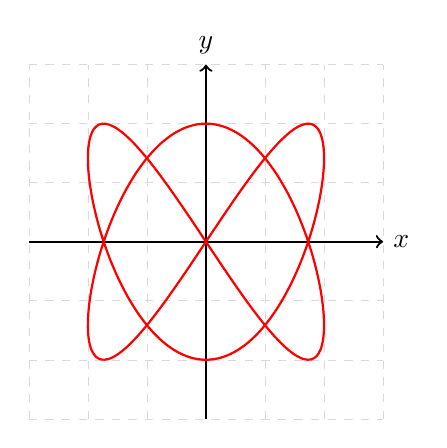
\begin{tikzpicture}[scale=1.5]
            \draw[help lines, color=gray!30, dashed, step=0.5] (-1.5,-1.5) grid (1.5,1.5);
            \draw[->,thick] (-1.5,0)--(1.5,0) node[right]{$x$};
            \draw[->,thick] (0,-1.5)--(0,1.5) node[above]{$y$};
            \draw[color=red,thick,domain=0:500, smooth, samples=150] plot ({sin(2*\x},{sin(3*\x)});
        \end{tikzpicture}
        \caption{Lissajous trajectory}
    \end{figure}

    The \textit{control.py} file is able to generate the controls to drive the trailing robot. These commands are generated by feedback linearization by controlling the robot in speed and heading. These controls leads to the trajectory in the simulator  as we could see on the \textsc{Figure}~\ref{fig:simulator_lissajous}

    \begin{figure}
        \centering
        \includegraphics[width=0.4\textwidth]{imgs/simulator_lissajous.png}
        \caption{Simulator's trajectory of the system}
        \label{fig:simulator_lissajous}
    \end{figure}

    Then the module \textit{mapping.py} allows to process the tubes including the trajectory of the trailing robot and the sledge. The tubes are then displayed in order to check that they seem to stick to the trajectory of the system.

    \begin{figure}[!htb]
        \centering
        \includegraphics[width=0.4\textwidth]{imgs/saturne_lissajous.png}
        \caption{Trailing vehicle enclosing tube}
        \label{fig:saturne_lissajous}
    \end{figure}

    \begin{figure}[!htb]
        \centering
        \includegraphics[width=0.4\textwidth]{imgs/magnetometer_lissajous.png}
        \caption{Magnetometer enclosing tube}
        \label{fig:magnetometer_lissajous}
    \end{figure}

    \begin{figure}[!htb]
        \centering
        \includegraphics[width=0.4\textwidth]{imgs/mapping_lissajous.png}
        \caption{Magnetometer enclosing tube}
        \label{fig:mapping_lissajous}
    \end{figure}